\colorlet{punct}{red!60!black}
\definecolor{background}{HTML}{EEEEEE}
\definecolor{delim}{RGB}{20,105,176}
\colorlet{numb}{magenta!60!black}

\Chapter{Tervezés}

\Section{Kinézet}

A kinézetet játékos, egyszerű és átláthatóra szeretném csinálni, valamint mindenhol vidám ikonokat és színvilágot szeretnék használni. Az oldal ikonja az alábbi lett, mivel a tesztek egy Game Boy-ként fognak megjelenni:

\begin{figure}[h]
    \centering
    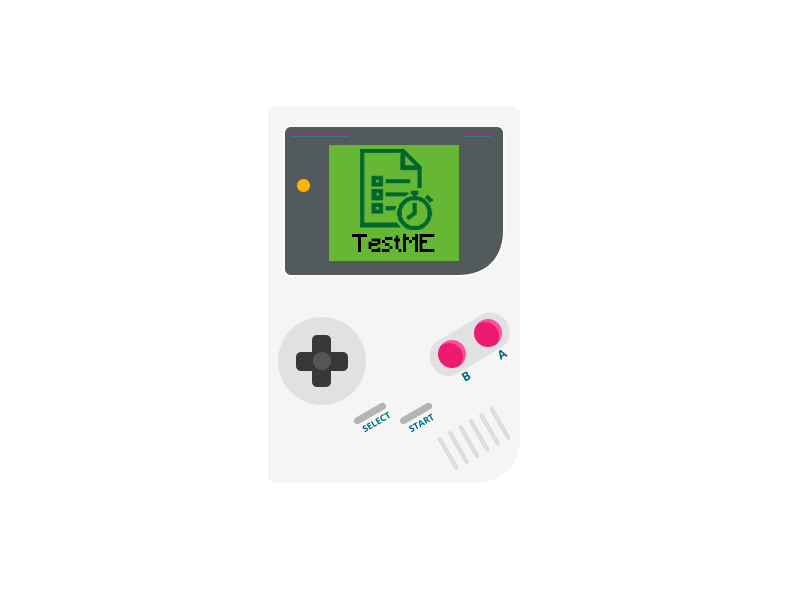
\includegraphics[height=5cm]{images/gameboy.png}
\end{figure}


Minden grafikus elemnél szeretném ha egységes lenne, így törekszem arra, hogy hasonló stílusú legyen minden. Az egyéb funkciókhoz vagy oldalakhoz társított ikonok is élénkek, színesek, egyszerűek és vidámak lesznek, hogy passzoljon az alkalmazáshoz. \newline

Az ikonokat a Flaticon nevű oldalról töltöttem le \cite{flaticon}.  \newline

Valamint Bootstrap-et szeretnék használni ami egy olyan keretrendszer, amely segít a weboldalak gyorsabb és könnyebb megtervezésében. HTML és CSS alapú tervezősablonokat tartalmaz a tipográfiához, űrlapokat, gombokat, táblázatokat, navigációt, modelleket stb. Ez segítene abban, hogy az oldalon egységes kinézetet hozhassak létre, valamit a Bootstrap CSS-je alkalmazkodik a telefonokhoz, táblagépekhez és asztali számítógépekhez is.

\Section{Az oldal felépítése}

A funkciók elrendezésének és felépítésének bemutatására képernyőterv vázlatot (magyarul drótváznak, angolul wireframe vagy mockup-nak is nevezzük) készítettem a MockFlow \cite{mockflow} nevű oldalon.
Elsődlegesen azt az oldalt mutatom be amivel mindenki először találkozik a megnyitáskor, ez pedig a bejelentkezési és regisztrációs felület.

\subsection{Bejelentkezés és regisztráció}

\begin{figure}[H]
    \centering
    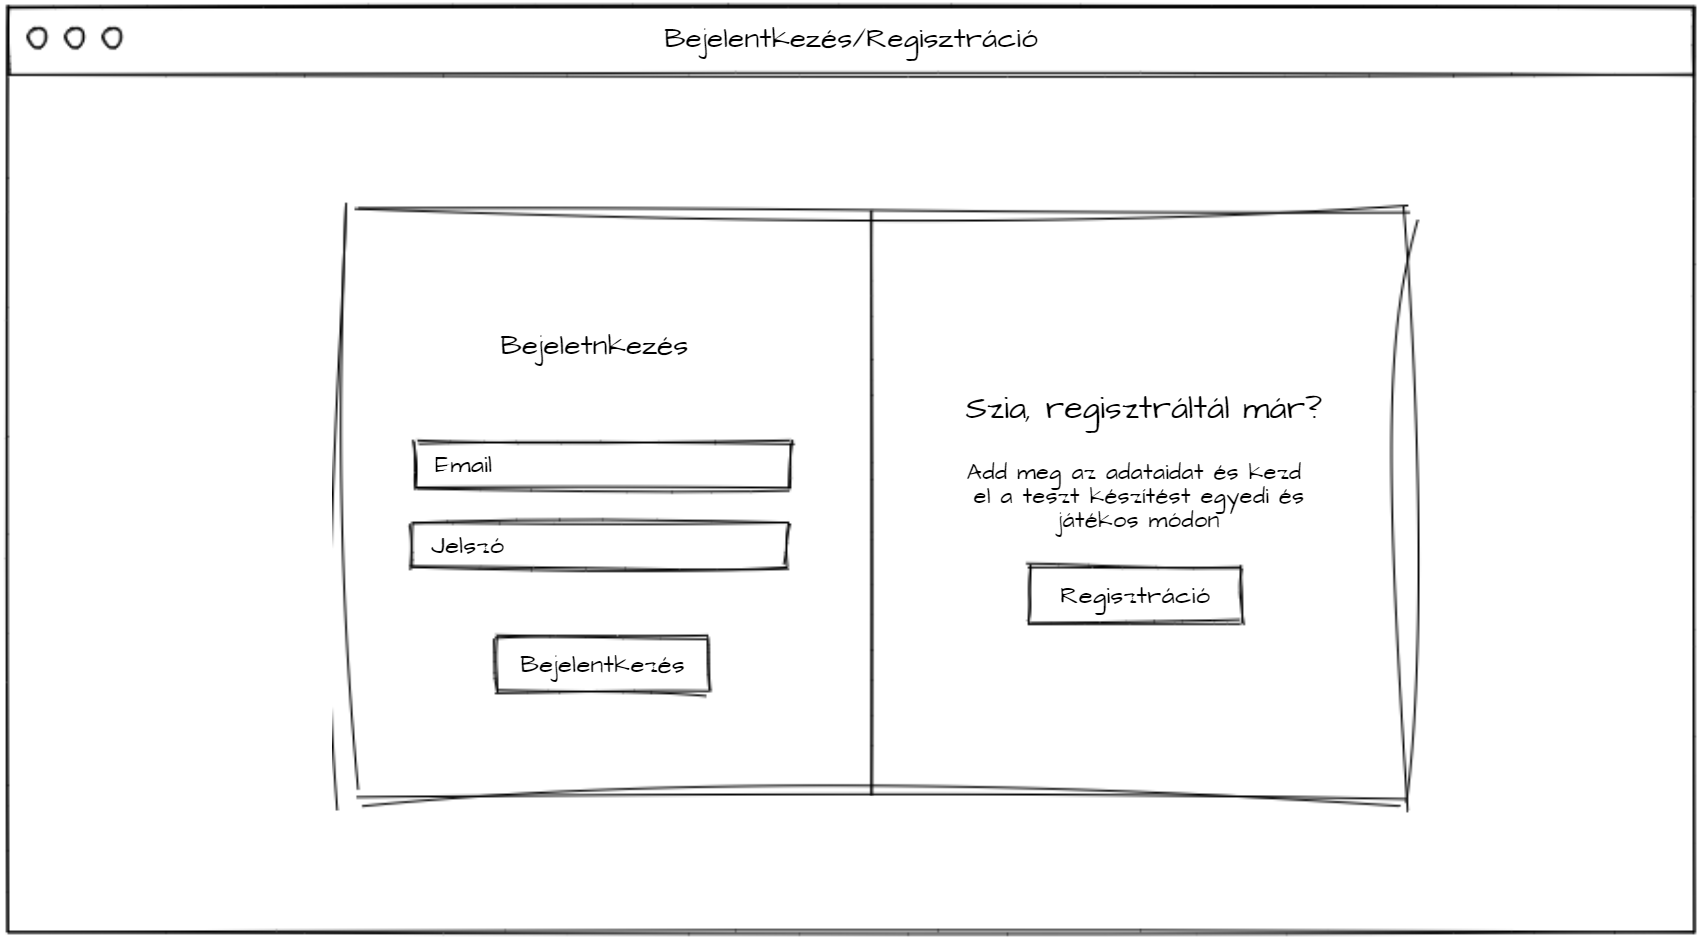
\includegraphics[width=\linewidth]{images/login_wireframe.png}
    \caption{Bejelentkezés}
    \label{fig:login_wireframe}
\end{figure}

Bejelentkezni \prettyref{fig:login_wireframe} email cím és jelszóval lehet.

\begin{figure}[H]
    \centering
    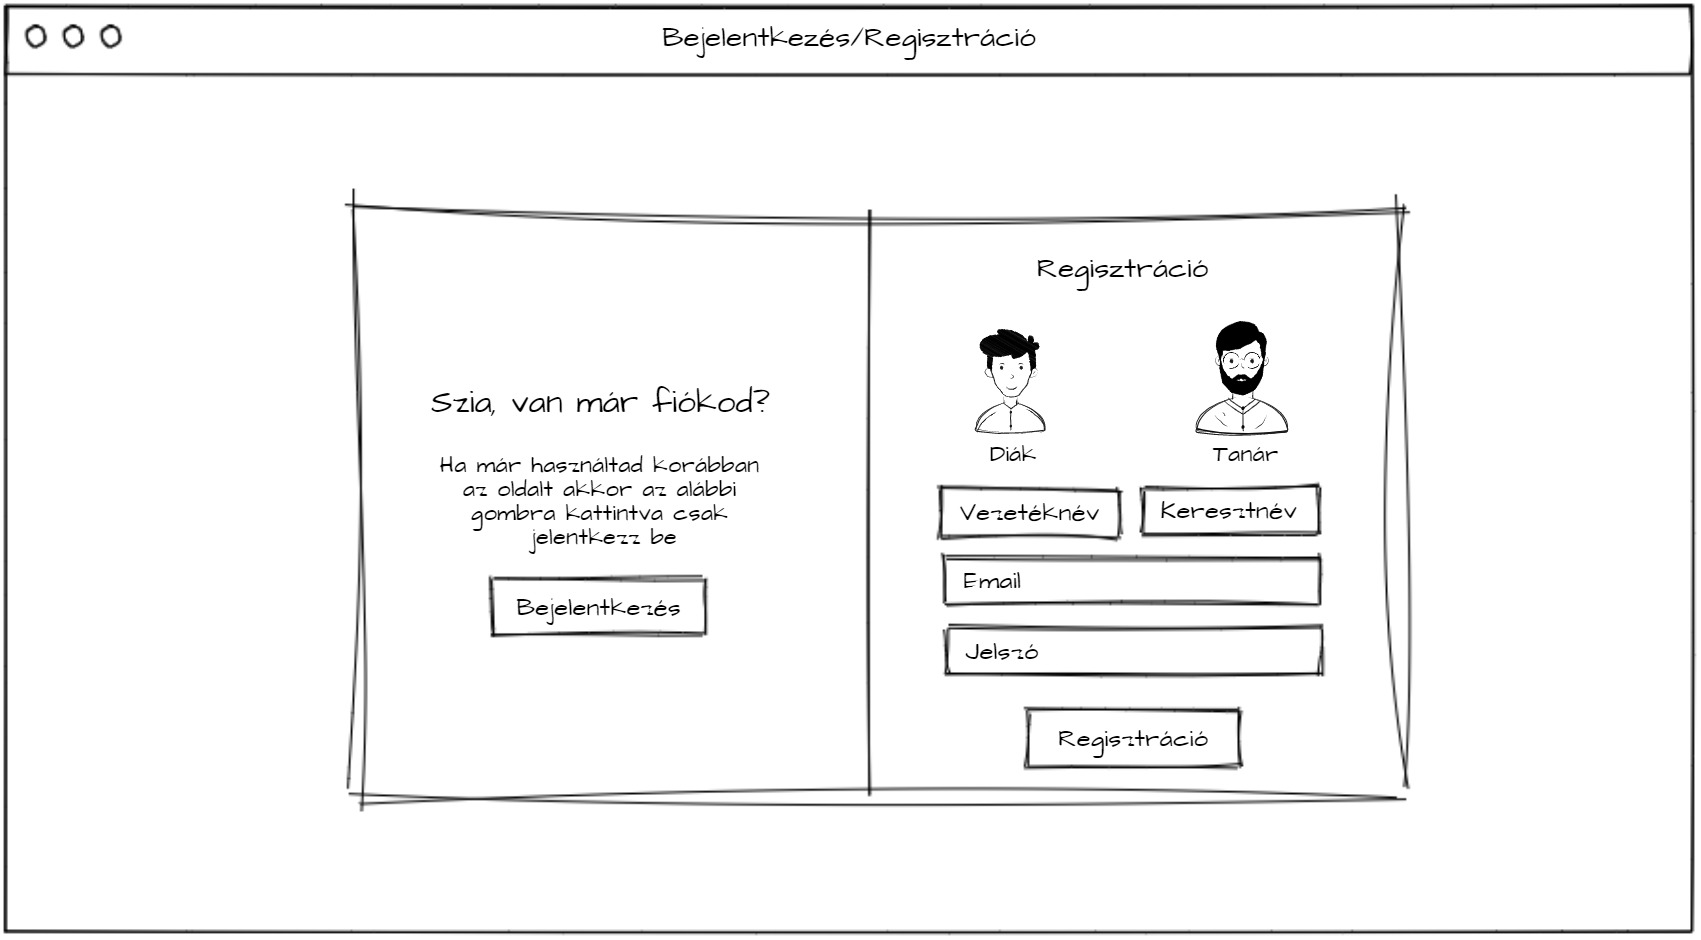
\includegraphics[width=\linewidth]{images/signin_wireframe.png}
    \caption{Regisztráció}
    \label{fig:signin_wireframe}
\end{figure}

Regisztrációkor \prettyref{fig:signin_wireframe} pedig ki kell választani, hogy tanár vagy diákként szeretnénk regisztrálni majd meg kell adni az alapvető adatokat.
Ezután, ha sikeresen beléptünk vagy regisztráltunk akkor hozzáférhetünk az oldalhoz.

\subsection{Főoldal}

\begin{figure}[H]
    \centering
    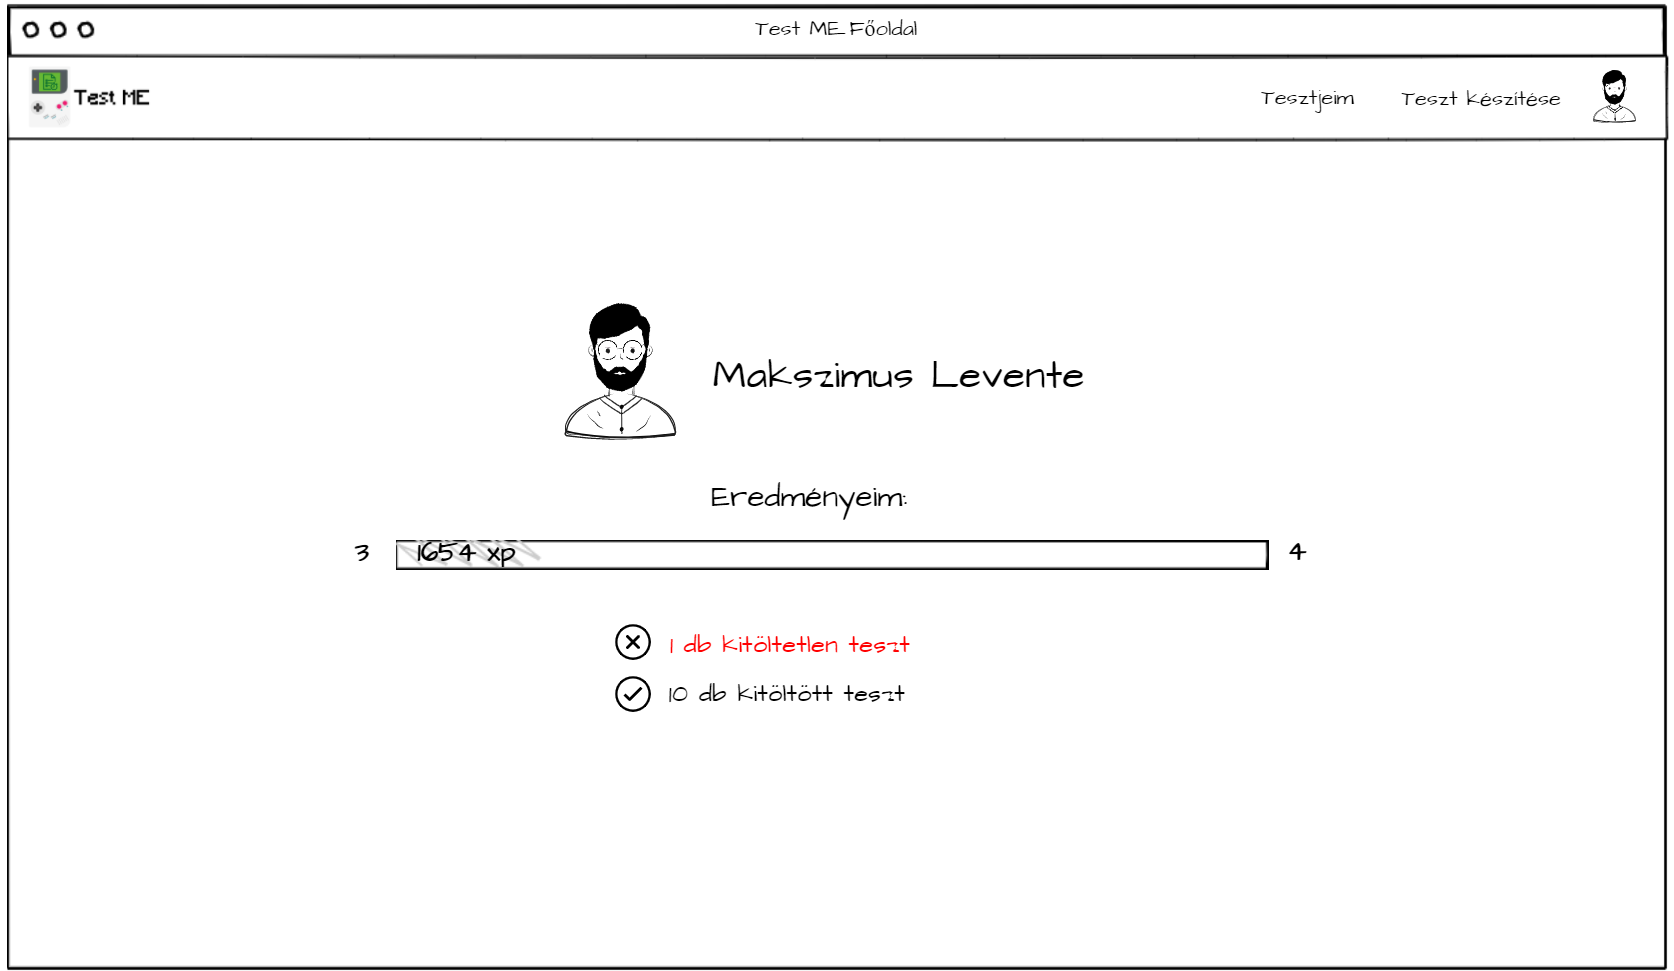
\includegraphics[width=\linewidth]{images/main_login_wireframe.png}
    \caption{Főoldal}
    \label{fig:main_page}
\end{figure}

Itt láthatjuk \prettyref{fig:main_page} a felhasználónevünket, hogy mennyi xp-vel rendelkezünk, hányas szintűek vagyunk és, hogy hány darab kitöltött és kitöltetlen tesztünk van még.

\subsection{Teszt készítés}

\begin{figure}[H]
    \centering
    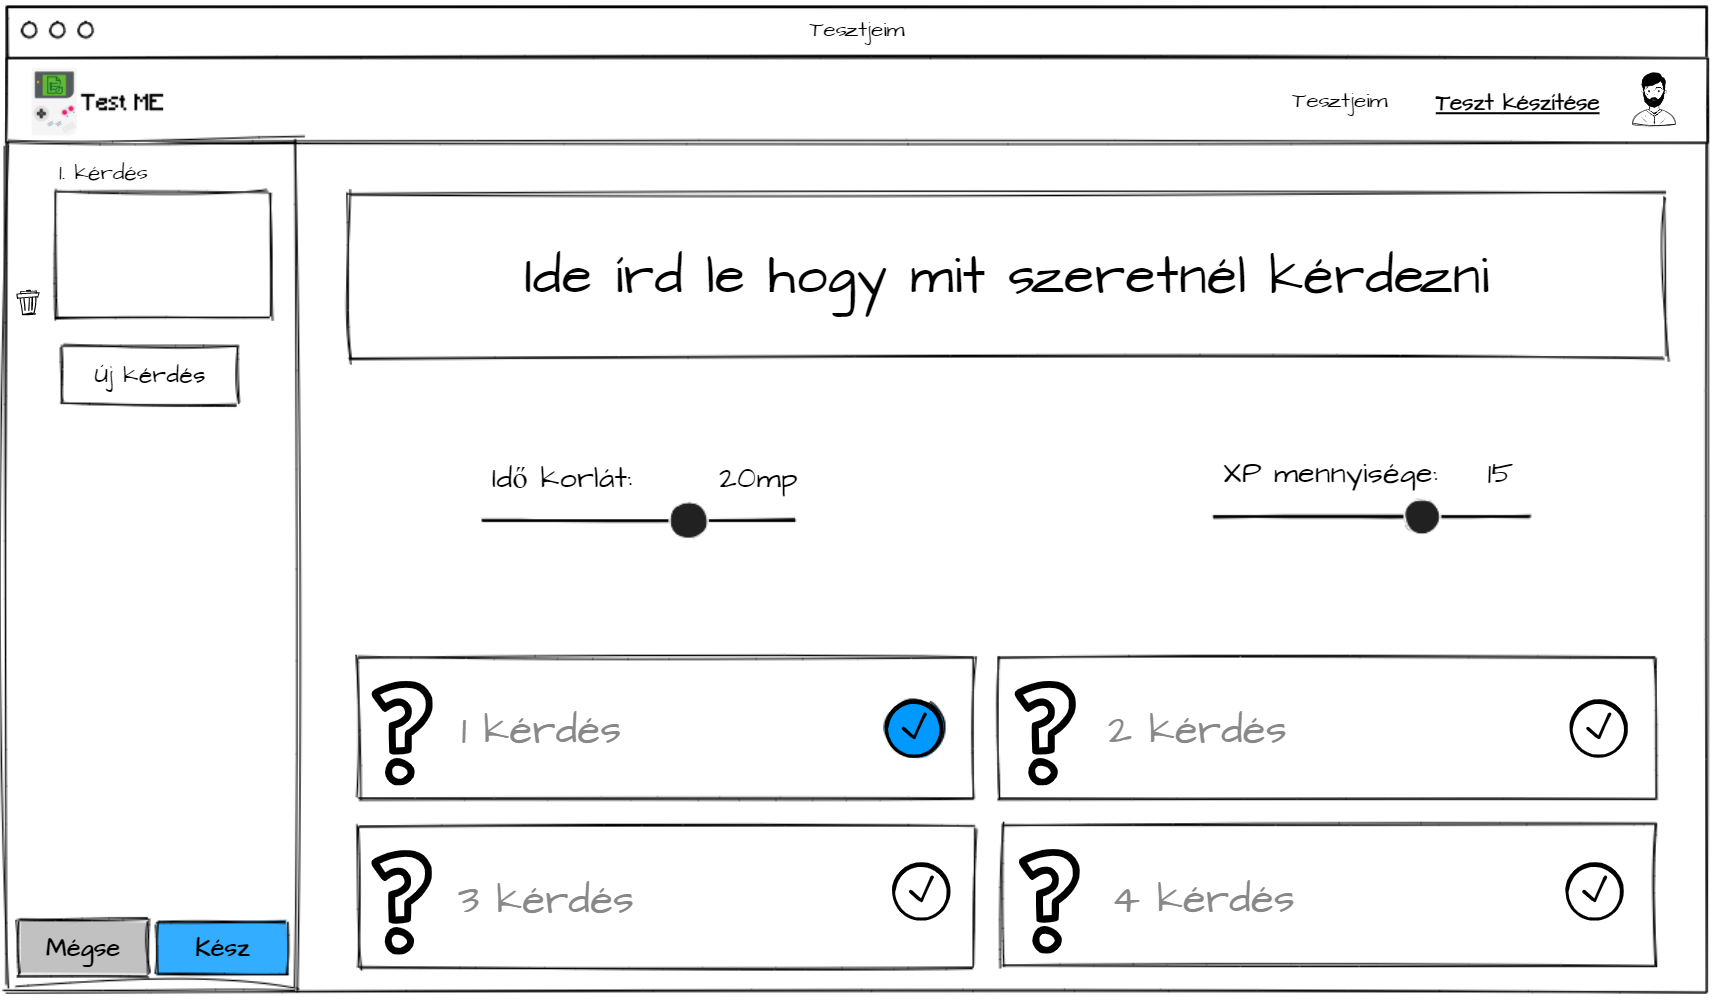
\includegraphics[width=\linewidth]{images/make_test_wireframe.png}
    \caption{Kvíz teszt készítés}
    \label{fig:new_quiz_question}
\end{figure}

Ezen a képen \prettyref{fig:new_quiz_question} a tesztkészítési felület látható. Egy tesztnél meghatározható maga a kérdés, ideje, illetve a jutalmazása, mely xp-ként van rögzítve. A választ kiválaszthatjuk az általunk írtak közül és beállíthatjuk melyik legyen a helyes megoldás.

\begin{figure}[H]
    \centering
    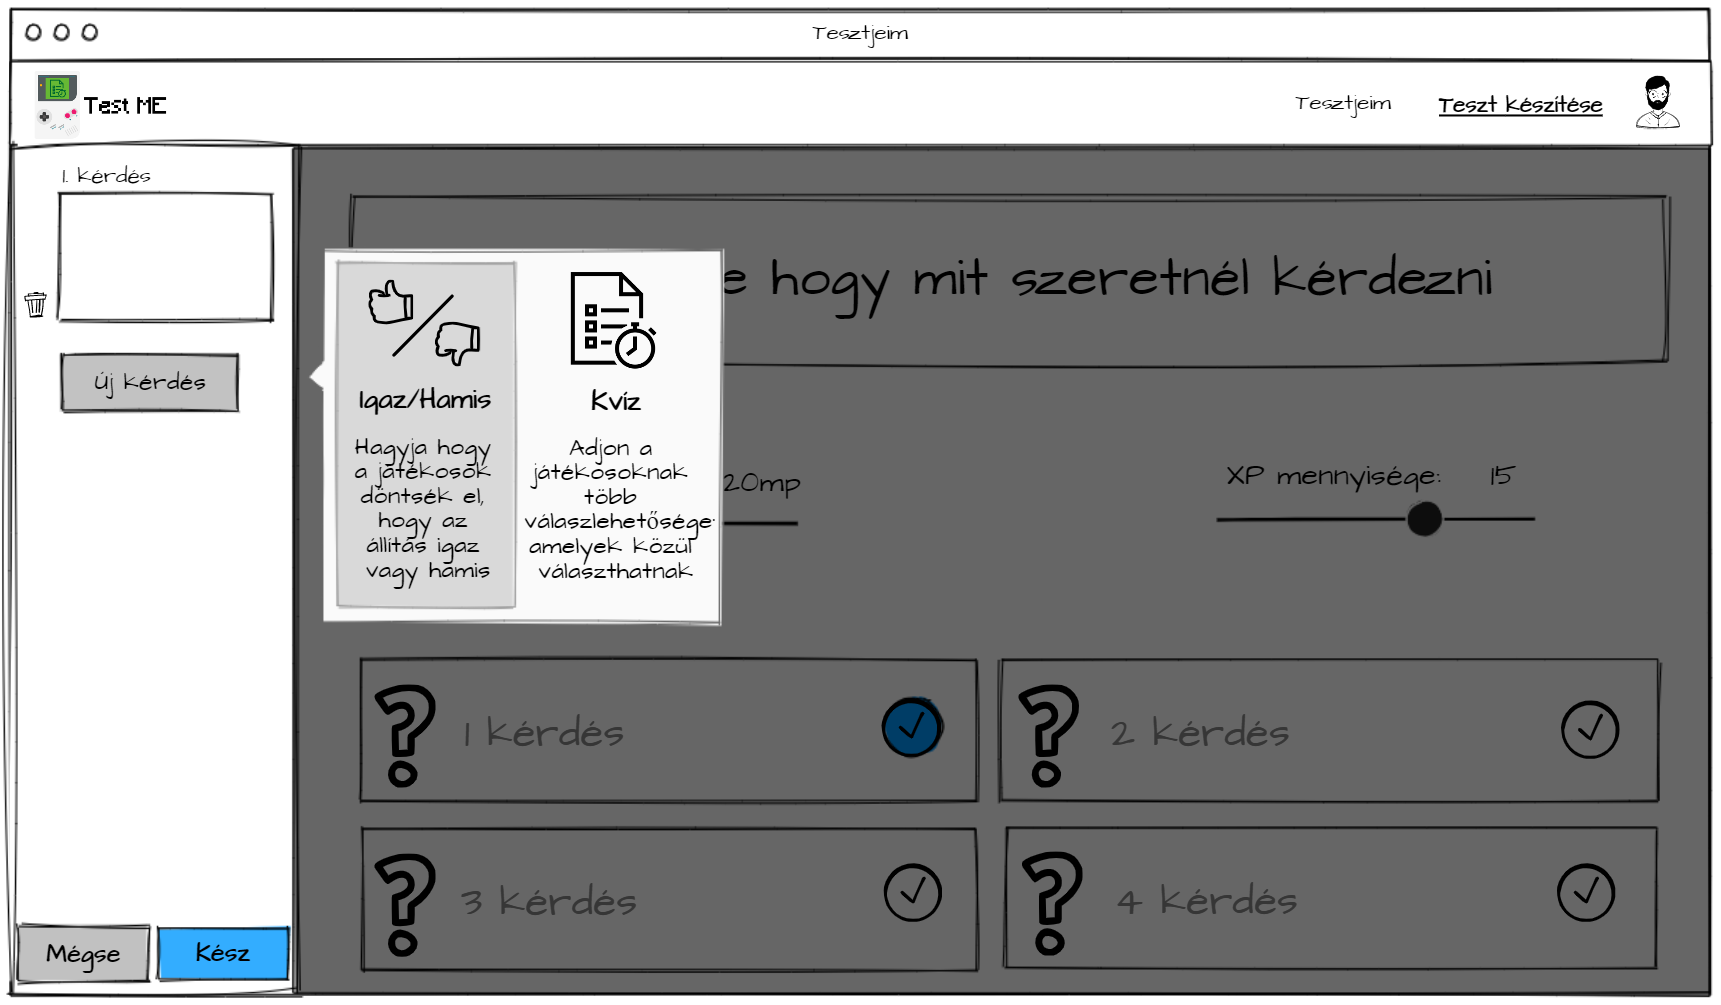
\includegraphics[width=\linewidth]{images/make_test2_wireframe.png}
    \caption{Új kérdés hozzáadása}
    \label{fig:new_question}
\end{figure}

Ezután ha elkészült a kérdés az "Új kérdés" gomb megnyomásával lehet hozzáadni a kérdések sorába. Itt választhatunk igaz/hamis, vagy kvíz típusú alternatíva közül, hogy milyet szeretnénk feltenni \prettyref{fig:new_question}.

\begin{figure}[H]
    \centering
    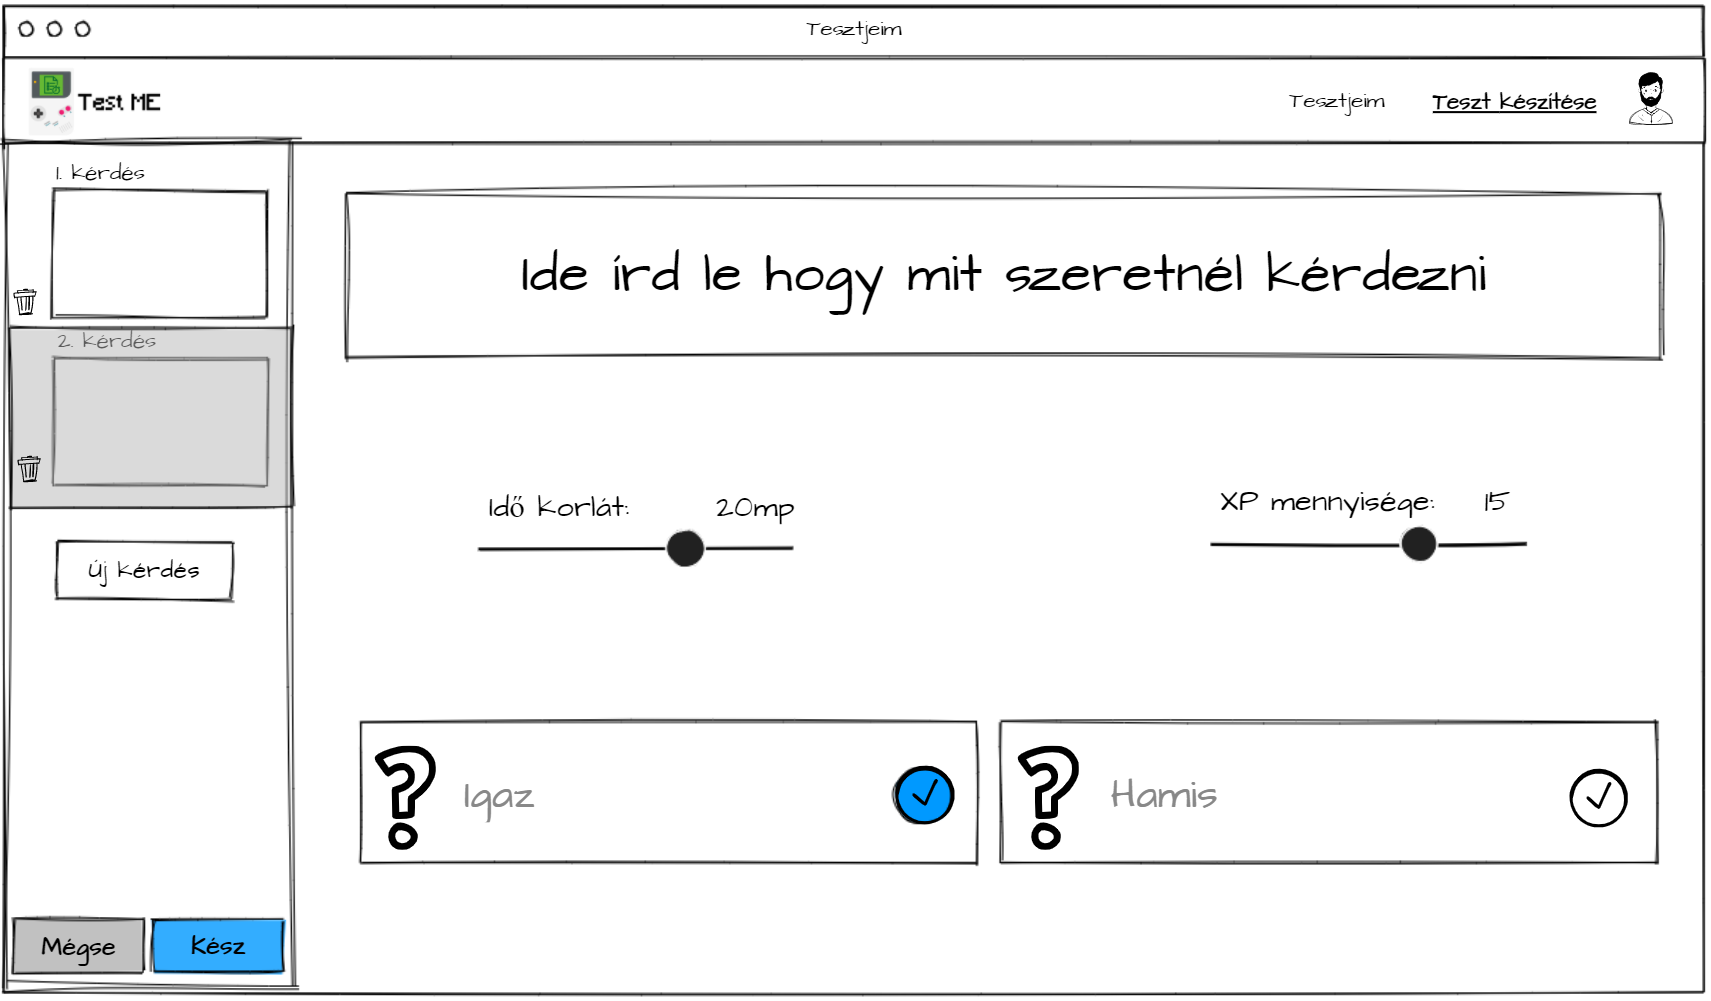
\includegraphics[width=\linewidth]{images/make_test3_wireframe.png}
    \caption{Igaz/hamis teszt készítése}
    \label{fig:test_true_false}
\end{figure}

Az igaz/hamis típusú kérdésnél csak annyi változik, hogy nem lehet válasz lehetőséget írni, csak egy állítást, amiről el kell dönteni, hogy valótlan vagy sem \prettyref{fig:test_true_false}.

\begin{figure}[H]
    \centering
    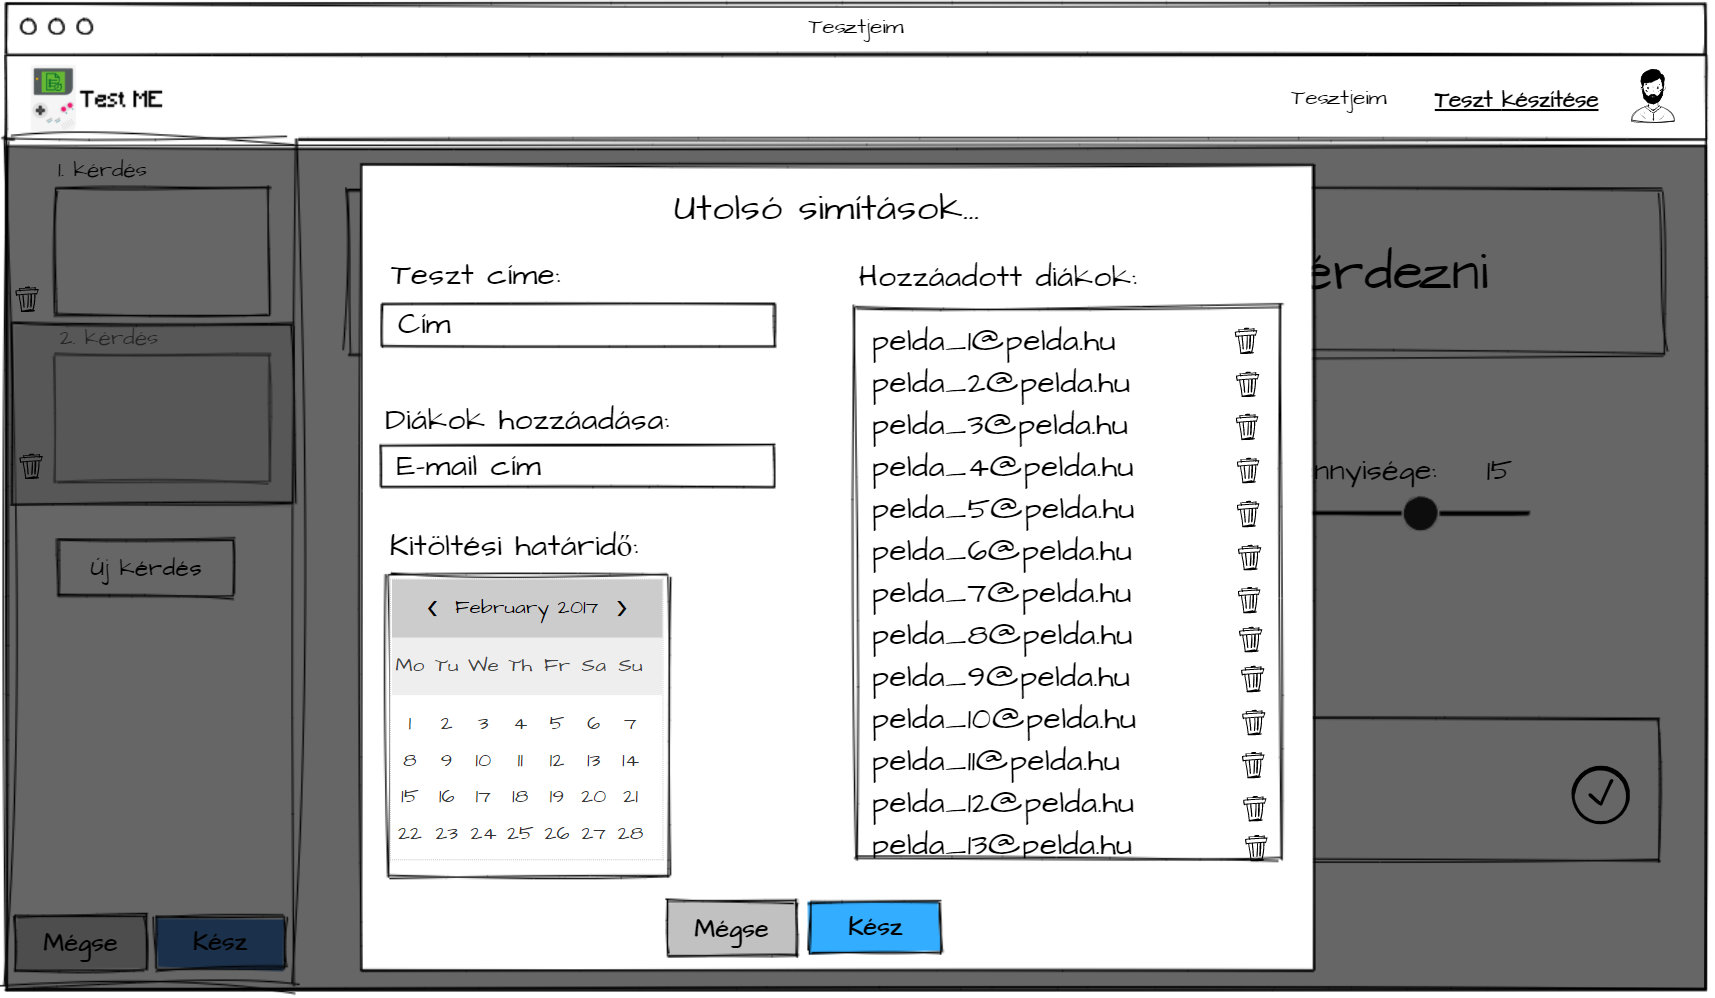
\includegraphics[width=\linewidth]{images/make_test4_wireframe.png}
    \caption{Adatok megadása és teszt elmentése}
    \label{fig:save_test}
\end{figure}

Az utolsó lépés pedig az, hogy adunk címet a tesztnek, ilyen névvel fog megjelenni majd a tanulóknak. Ezután hozzáadunk tetszőleges számú diákot akiktől szeretnénk, hogy töltsék ki, egy kitöltési határidőt és elkészült a tesztünk \prettyref{fig:save_test}.

\subsection{Saját tesztek}
\begin{figure}[H]
    \centering
    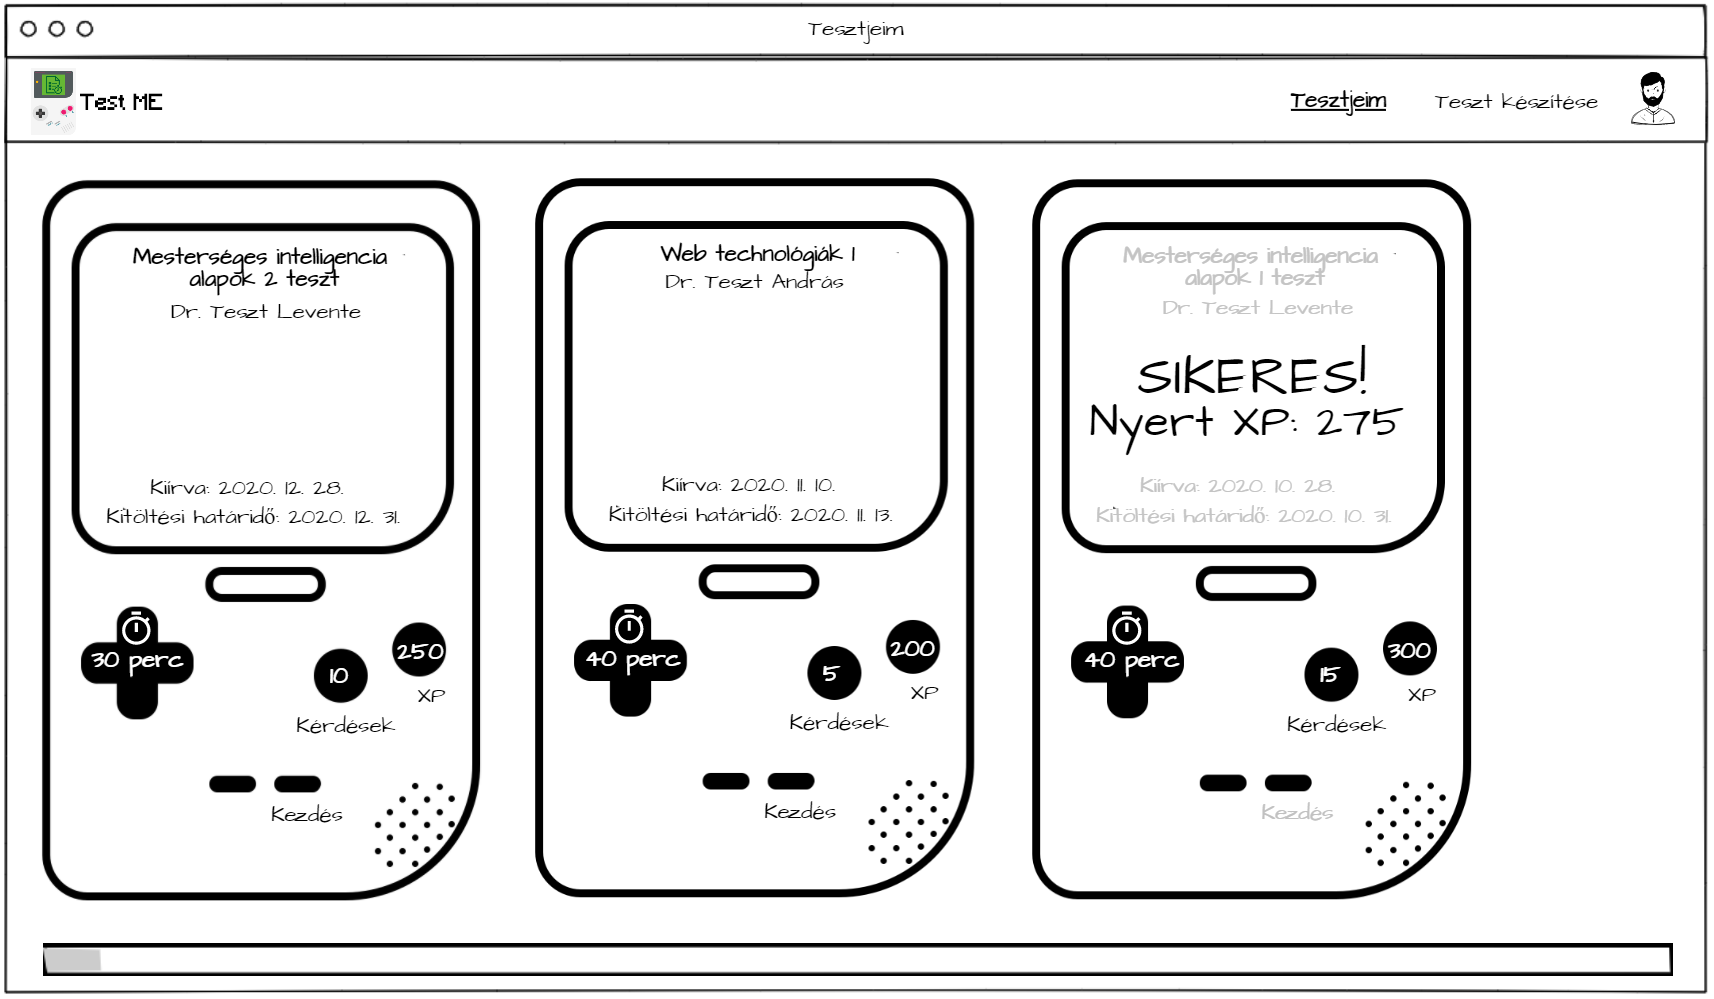
\includegraphics[width=\linewidth]{images/my_tests_wireframe.png}
    \caption{Felhasználóhoz rendelt tesztek}
    \label{fig:my_tests}
\end{figure}

Ezen a képen \prettyref{fig:my_tests} a diákhoz rendelt teszteket látjuk. Itt azok az adatok láthatóak amiket tesztkészítéskor adtunk meg. Tehát a kitöltési határidő, a teszt címe, mennyi idő van rá, hány kérdés van és, hogy mennyi pontot lehet szerezni. Ezenkívül láthatjuk még, hogy mikor lett kiírva és egy kezdés gombot amivel kitölthetjük.

\subsection{Teszt kitöltése}

\begin{figure}[H]
    \centering
    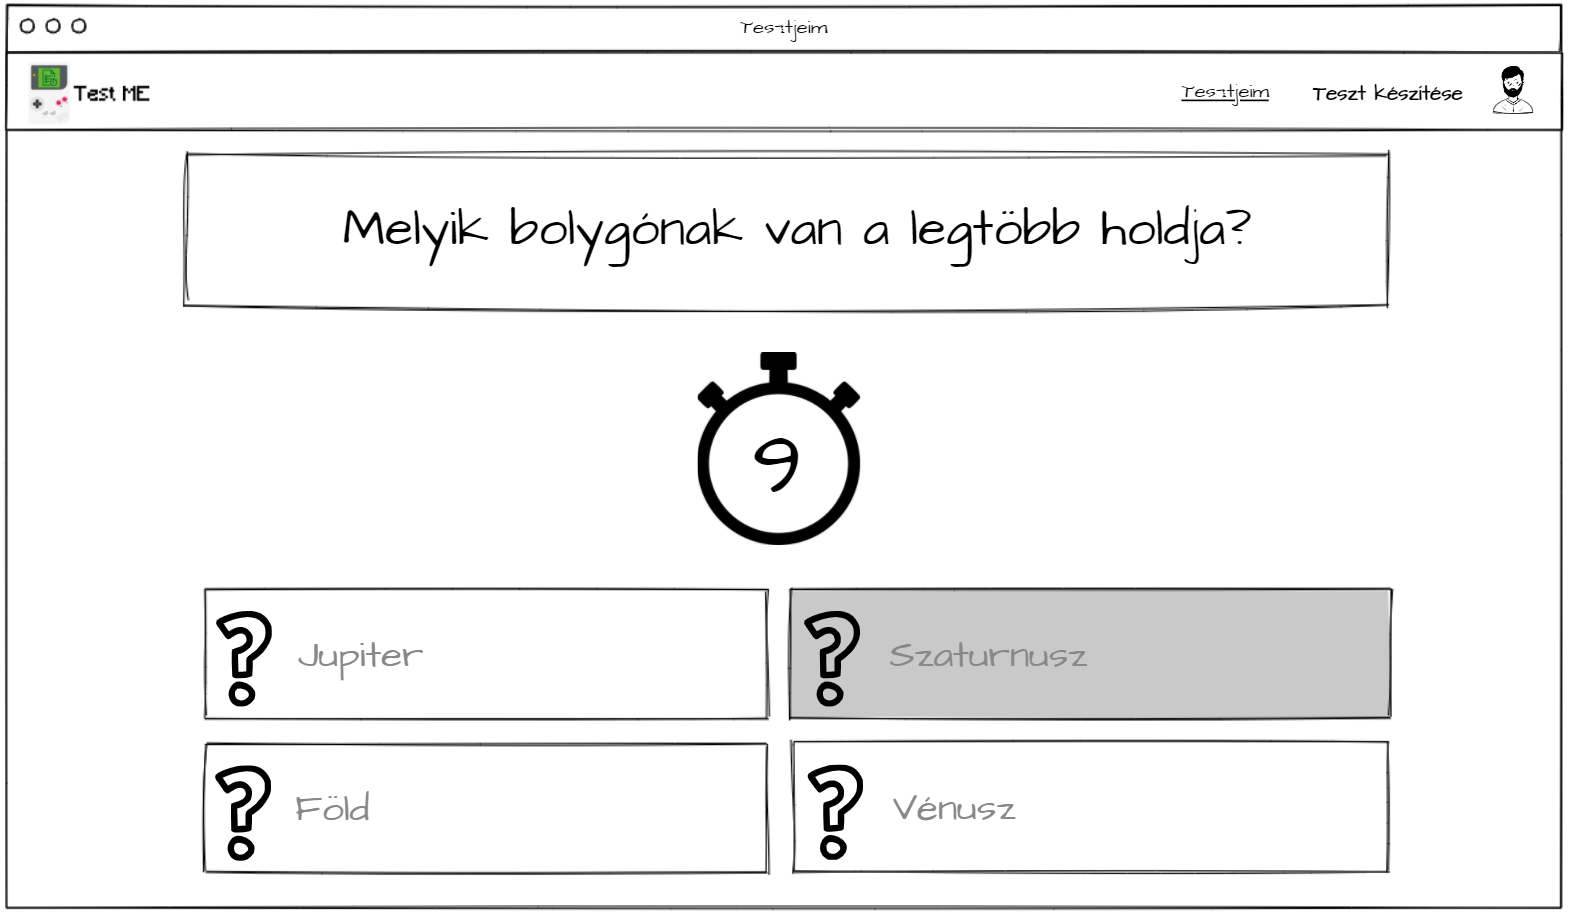
\includegraphics[width=\linewidth]{images/test1_wireframe.png}
    \caption{Feltett kérdés}
    \label{fig:test_question}
\end{figure}

Itt \prettyref{fig:test_question} egy kérdést látható teszt indítás után. Minden kérdésnél egy stopper órában láthatjuk, hány másodpercünk van még válaszolni.

\begin{figure}[H]
    \centering
    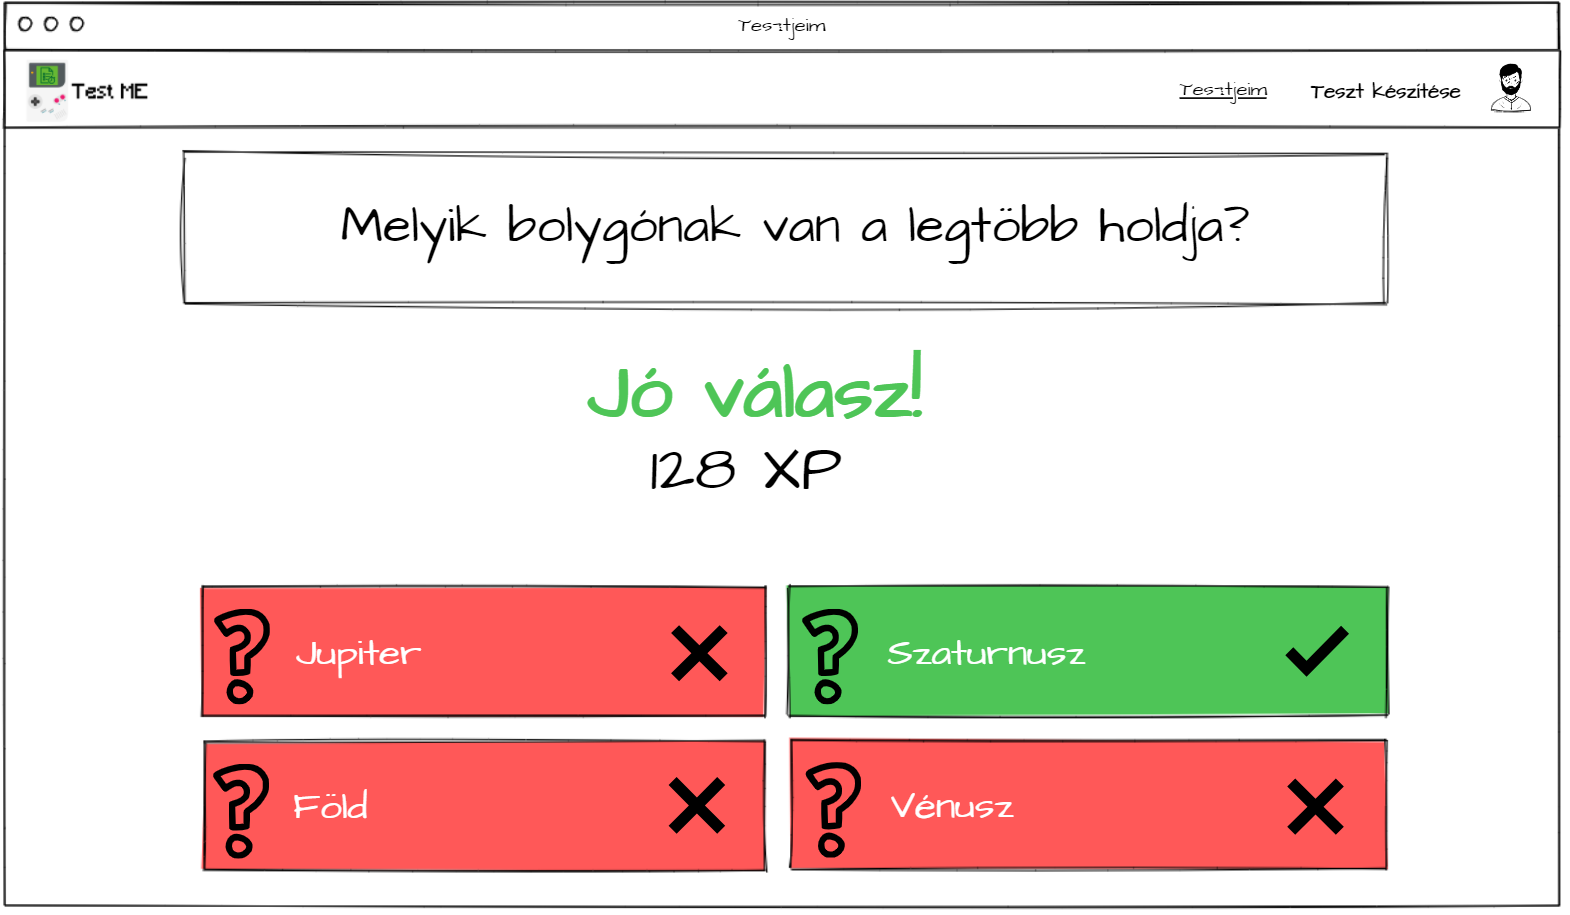
\includegraphics[width=\linewidth]{images/test2_wireframe.png}
    \caption{Válasz a kérdésre}
    \label{fig:test_answer}
\end{figure}

Válasz adás után pedig láthatjuk \prettyref{fig:test_answer}, hogy ha válaszolunk egy kérdésre akkor melyik volt a jó.

\begin{figure}[H]
    \centering
    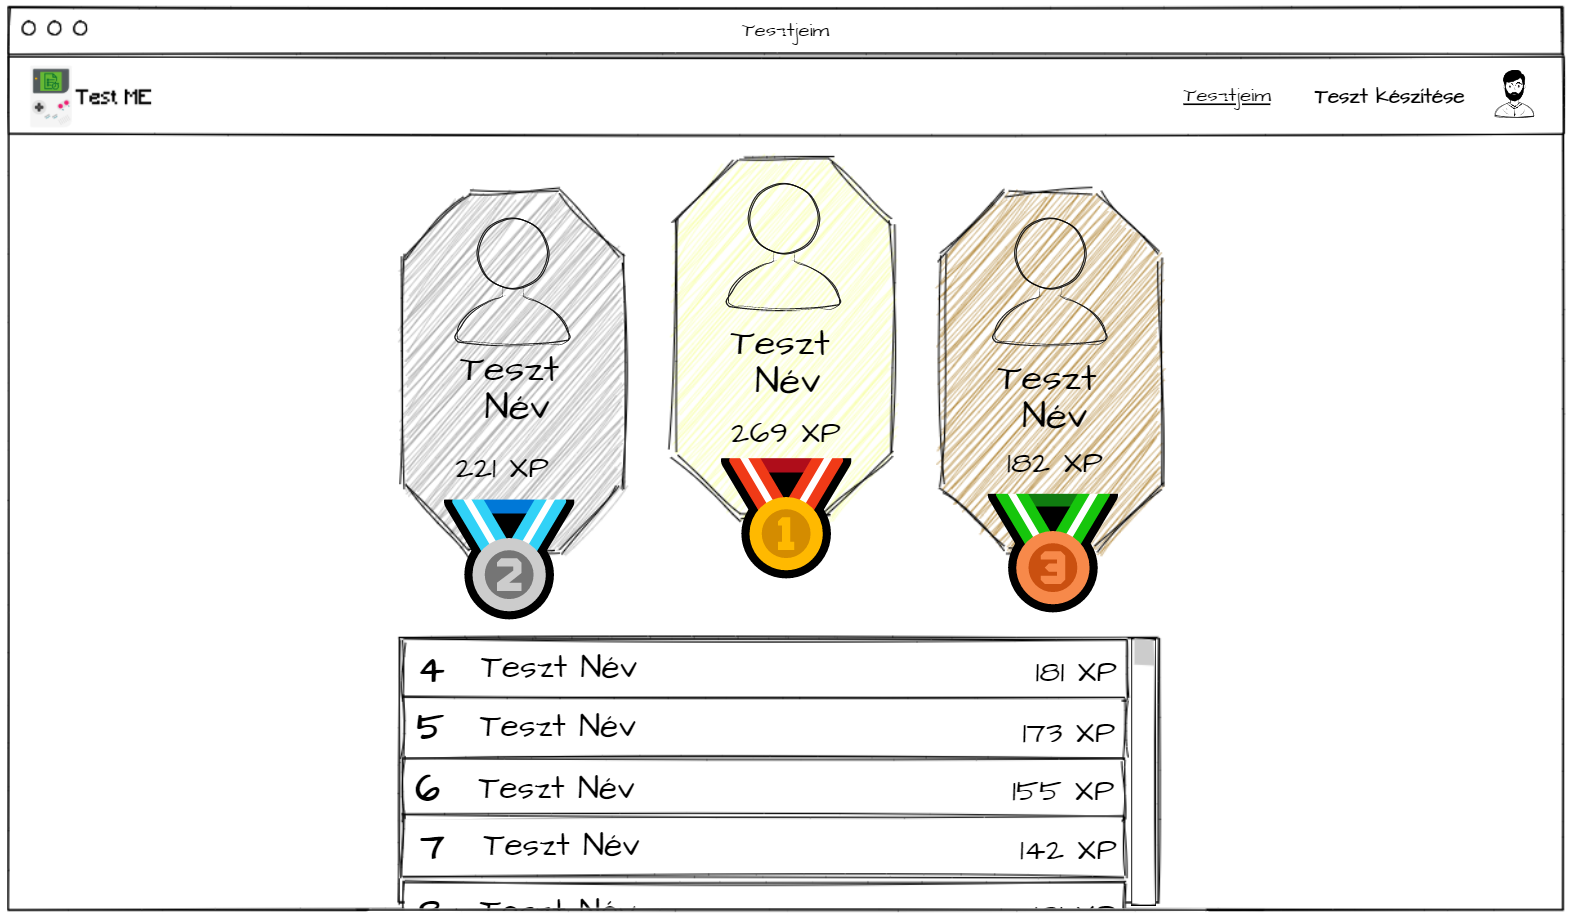
\includegraphics[width=\linewidth]{images/test3_wireframe.png}
    \caption{Teszt eredmény}
    \label{fig:test_finished}
\end{figure}

Miután válaszoltunk minden kérdésre, megnézhetjük mennyi pontot gyűjtöttünk és a kitöltők közül, kik lettek a legjobbak. \prettyref{fig:test_finished}


\Section{Funkciók}

\begin{itemize}
    \item {Bejelentkezés/Regisztráció}
          \begin{addmargin}[\parindent]{0pt}
              Az oldalon lévő minden funkciót csak regisztráció vagy bejelentkezés után lehet használni. Ez azért fontos hiszen, csak így lehet a felhasználónak tesztet küldeni és kitöltés után hozzáadni a profiljához a pontokat és megjeleníteni a nevét a ranglistán. Az weboldal megnyitásakor a felhasználónak be kell jelentkeznie, egy helyes e-mail címmel és egy kellően biztonságos jelszóval vagy regisztrálnia kell, ha használni szeretné az oldalt.
          \end{addmargin}
    \item {Tesztkészítés}
          \begin{addmargin}[\parindent]{0pt}
              Kahoot!-hoz hasonló teszt készítési felületet szeretnék létrehozni ahol az elkészített teszteket hozzá lehet rendelni diákokhoz és ezután kitölthetik azokat.

              A két következő funkció az egyik legalapvető eleme a játékosításnak, viszont egy jó teszt nélkül értékét vesztik. A fejlődés és a teljesíteni vágyás a belső motiváció számunkra, hogy kihívásokat teljesítsünk. Viszont kihívások nélkül a pontok és a jelvények vagy bármi féle jutalmak feleslegesnek tűnnek. Emiatt fontos, hogy a tesztek kellő kihívást nyújtsanak, hogy aztán a jó eredménnyel járó hasznokat is jutalomnak érezzük.
          \end{addmargin}
    \item {Pontgyűjtés}
          \begin{addmargin}[\parindent]{0pt}
              Minden regisztrált felhasználó rendelkezik majd egy szinttel és egy bizonyos pontszámmal, amelyet a tesztek kitöltésével szerezhetnek.
          \end{addmargin}
    \item {Ranglista}
          \begin{addmargin}[\parindent]{0pt}
              Ranglista a teszt teljes kitöltését követően alakul ki a legtöbbet szerzett pontok alapján.
          \end{addmargin}
    \item {Tesztek diákokhoz rendelése}
          \begin{addmargin}[\parindent]{0pt}
              Teszt létrehozása során email cím vagy valamilyen más egyedi azonosító segítségével hozzá lehetne rendelni diákokhoz a tesztet és így értesülnének róla hogy ki kell tölteniük.
          \end{addmargin}
    \item {Összes hozzárendelt teszt megtekintése}
          \begin{addmargin}[\parindent]{0pt}
              Diákként meg lehet nézni az összes olyan tesztet amit valaki hozzá rendelt a profilhoz. És ezzel együtt a régiek eredményét is azért, hogy lássuk, hogy sikerült mindenkinek.
          \end{addmargin}
\end{itemize}

\Section{Adatmodell}
\label{Adatmodell}

Az adatokat egyed-kapcsolat diagrammon ábrázoltam így a teljes kép könnyebben áttekinthető ezen rendszervázlat alapján.

\begin{figure}[H]
    \centering
    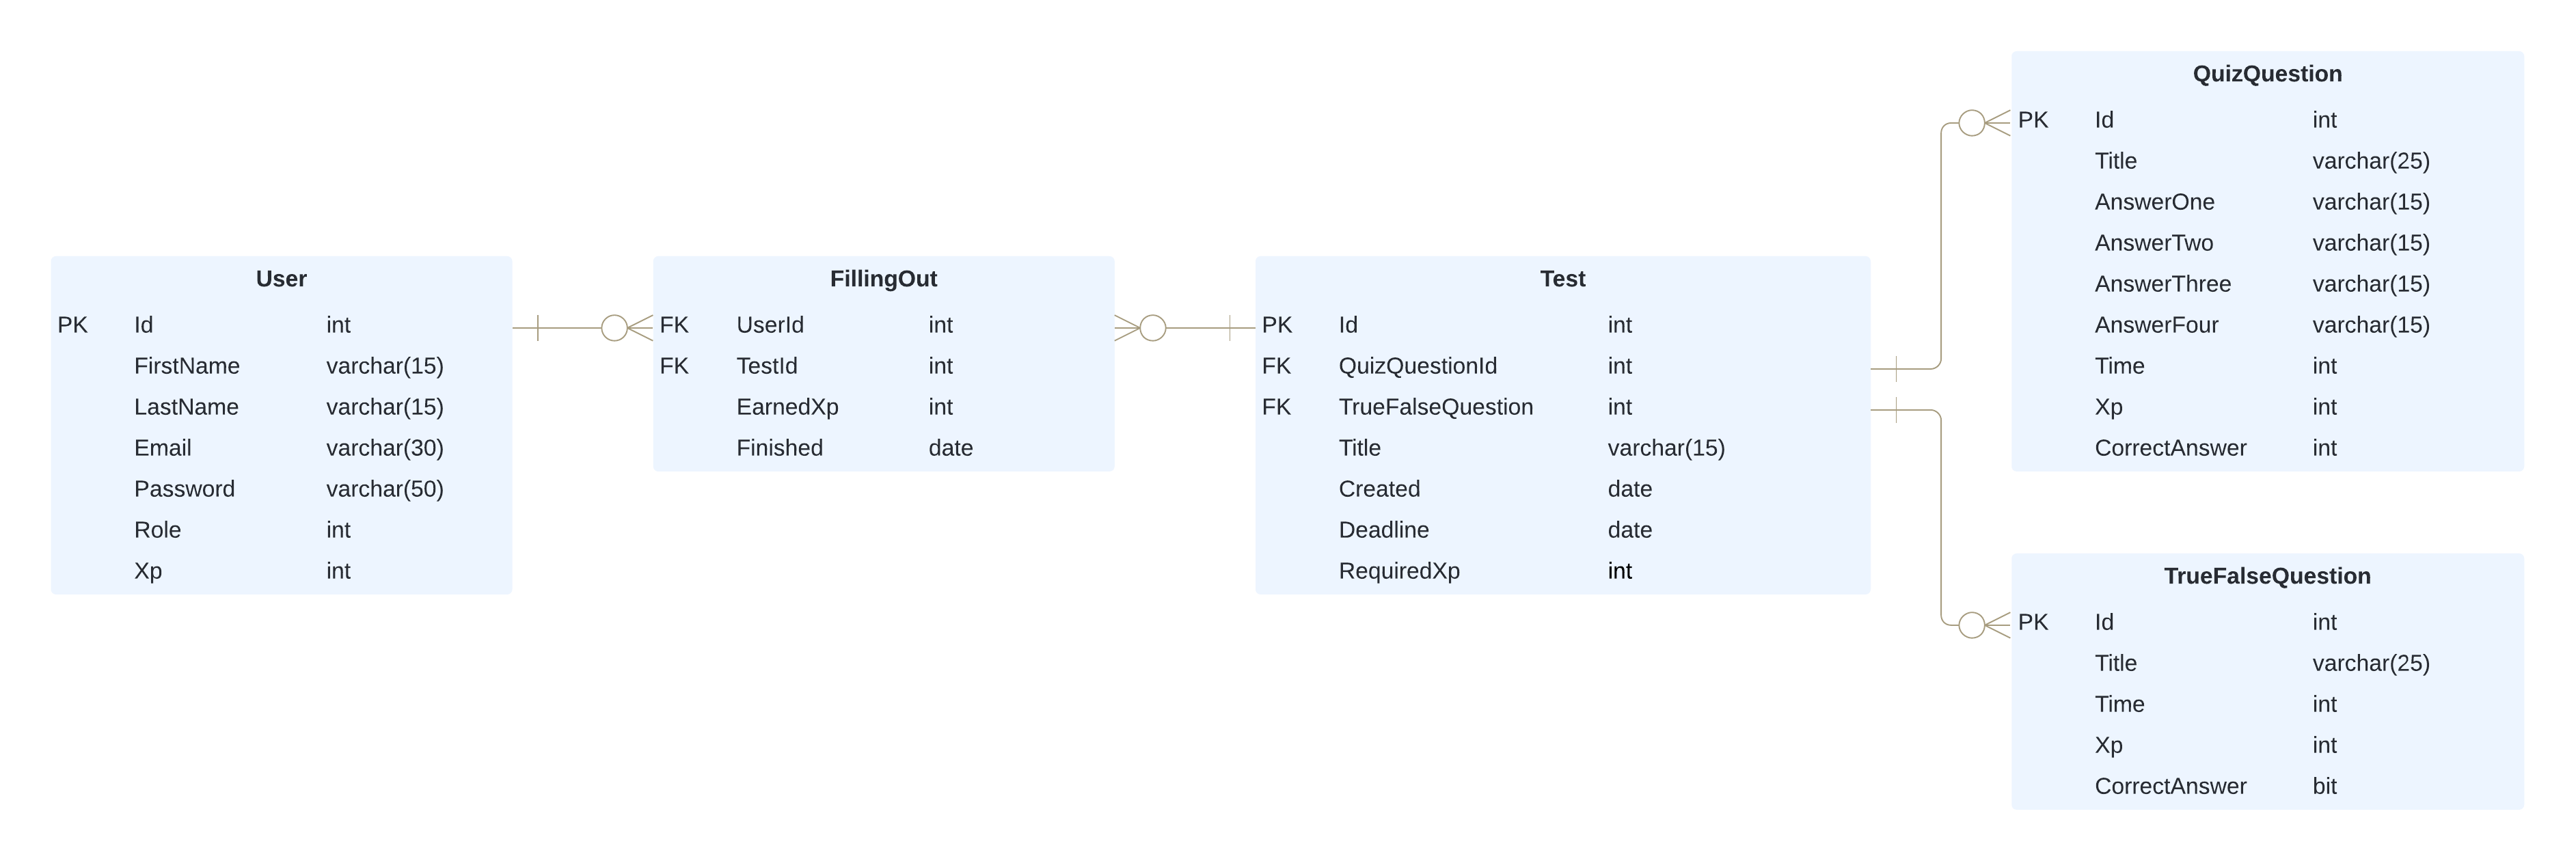
\includegraphics[width=\linewidth]{images/TestME_ER.png}
    \caption{ER modell}
    \label{fig:TestME_ER}
\end{figure}

A séma diagram \prettyref{fig:TestME_ER} az alábbi táblákat tartalmazza:
\begin{itemize}
    \item {User}
          \begin{addmargin}[\parindent]{0pt}
              Ez a tábla egy felhasználót reprezentál akinek az alap adatait bekérjük regisztrációkor, ilyen például a keresztnév, vezetéknév, email cím, jelszó. Majd ezen felül még van regisztráció dátuma és, hogy visszaigazolta-e az e-mail címét. Valamint meg kell határoznia milyen szerepkörben szeretné használni az oldalt és miután töltött ki tesztet, növekedni fog az xp-je mennyisége így van egy Xp adattag is.
          \end{addmargin}

    \item {Test}
          \begin{addmargin}[\parindent]{0pt}
              A Test tábla egy felhasználó által készített tesztet reprezentál. Egy teszten belül két típusú kérdés lehet az egyik a kvíz a másik az igaz/hamis. Ezenkívül benne van a teszt leírása, a készítő azonosítója, a teszt címe, hogy mikor készült és hogy mi a kitöltési határidő.
          \end{addmargin}

    \item {Question}
          \begin{addmargin}[\parindent]{0pt}
              A Question egy kérdés adatait tárolja amibe beletartozik a kérdés szövege, a négy válasz, az idő, hogy mennyi pontot ér és, hogy melyik a helyes válasz.
          \end{addmargin}

    \item {UsersTest}
          \begin{addmargin}[\parindent]{0pt}
              Ez egy kapcsolótáblát képez a Test és a User tábla között. A kapcsolótábla azonosítója a két idegen kulcsból képzett összetett kulcs lesz. Tehát ebbe benne lesz a Test és User tábla idegen kulcsa. Valamint itt tárolódik el, hogy felhasználó kitöltötte már a tesztet és ha igen akkor mikor és mennyi pontot ért el. Ez a legtöbbet használt tábla az oldal működése során, hiszen innen szedjük ki az adatokat, ha megszeretnénk nézni milyen tesztjeink vannak és ha kitöltjük itt módosítjuk a pontot és a dátumot.
          \end{addmargin}

    \item {Answer}
          \begin{addmargin}[\parindent]{0pt}
              Ez a tábla egy kérdés válaszát tárolja el. Ebben benne van a kérdés és a UsersTest tábla id-ja, emellett, hogy meny idő alatt válaszolt a felhasználó a kérdésre és, hogy mi volt a válasza.
          \end{addmargin}
\end{itemize}

\Section{API}
\label{API}

Az alábbi endpointokat szeretném használni az alkalmazásban:

\begin{itemize}
    \item{api/users:}
          \begin{addmargin}[\parindent]{0pt}
            Ezen az endpoint-on tudunk majd lekérni egy felhasználót bejelentkezéskor, elmenteni és lekérni a felhasználó session-jét, az id-ját és az email címét. Valamint regisztrációkor ide szeretném elküldeni a felhasználó bejelentkezési adatait és azt, hogy ki szeretne jelentkezni.
          \end{addmargin}

    \item{api/tests:}
          \begin{addmargin}[\parindent]{0pt}
            Ha a diák ki akarja tölteni a tesztet, innen tudjuk majd lekérni a kérdésekkel együtt. Illetve, ha valaki készít egyet akkor ide lehet elküldeni az újat.
          \end{addmargin}

    \item {api/questions:}
          \begin{addmargin}[\parindent]{0pt}
            Egy teszthez tartozó kérdéseket külön kontroller kezeli és ide kerül majd elküldésre teszt létrehozáskor.
          \end{addmargin}
          
    \item {api/answers:}
        \begin{addmargin}[\parindent]{0pt}
            Teszt kitöltés után ide érkeznének a válaszok.
        \end{addmargin}
    
    \item {api/users-tests:}
          \begin{addmargin}[\parindent]{0pt}
            Ha egy diák meg akarja nézni a saját tesztjeit, hogy miket kell kitöltenie vagy miket töltött ki eddig, akkor azt innen tudjuk majd lekérdezni. Ezáltal kiírathatjuk őket a "Tesztjeim" menüpont alatt, hogy befejezték-e már és mennyi pontot kaptak általa. Emellett a kitöltött és kitöltetlen tesztek száma is innen jön ami a főoldalon látható. Kitöltés után pedig itt kerül módosításra az xp adattag, a teszt után kapott pont alapján.
          \end{addmargin}
\end{itemize}